 

\documentclass[12pt]{article}
%%%%%%%%%%%%%%%%%%%%%%%%%%%%%%%%%%%%%%%%%%%%%%%%%%%%%%%%%%%%%%%%%%%%%%%%%%%%%%%%%%%%%%%%%%%%%%%%%%%%%%%%%%%%%%%%%%%%%%%%%%%%%%%%%%%%%%%%%%%%%%%%%%%%%%%%%%%%%%%%%%%%%%%%%%%%%%%%%%%%%%%%%%%%%%%%%%%%%%%%%%%%%%%%%%%%%%%%%%%%%%%%%%%%%%%%%%%%%%%%%%%%%%%%%%%%
\usepackage{amsfonts}
\usepackage{eurosym}
\usepackage{geometry}
\usepackage{amsmath,amsthm,amssymb}
\usepackage{graphicx}
\usepackage{comment}
\usepackage{adjustbox}
\usepackage{array}
\usepackage{multirow}
\usepackage{subcaption}
\usepackage{pifont}
\usepackage{amssymb}
\usepackage{comment}
\usepackage[utf8]{inputenc}
\usepackage{setspace}
\usepackage[hang, flushmargin, bottom]{footmisc}
%\usepackage[backend=biber,style=apa,url=false,isbn=false, extra = false]{biblatex}

%\addbibresource{references.bib}
\usepackage{footnotebackref}
\usepackage{xcolor}
\usepackage{hyperref}
\usepackage{booktabs}
\usepackage{pifont}
\usepackage{caption}
\usepackage{float}


\setlength{\textfloatsep}{5pt}
\captionsetup{font=normalsize}
\newcommand{\cmark}{\ding{51}}
\def\sym#1{\ifmmode^{#1}\else\(^{#1}\)\fi}
\renewcommand{\thetable}{\Roman{table}}
\geometry{verbose,tmargin=.5in,bmargin=.7in,lmargin=.7in,rmargin=.7in,nomarginpar}
\makeatletter

\begin{document}




\title{Meeting 24th of june}

\maketitle

In this document I will present what we are learnign from out empirical work. 

\section{IE 0}

Figure \ref{fig:ie0_0} shows the increase of requests over time. The increase is smooth with the exception of the year 2009 to 2010 that almost doubles. Probably there was a regulatory change. 
On average consumers make 10.5 requests for different financial products. 

CHECK WHY THE INCREASE IS SO BIG FROM 2009 TO 2010.

Important to note that individuals 
\begin{figure}[H]
\caption{}
\label{fig:ie0_0}
\centering{}%
\begin{tabular}{cc}
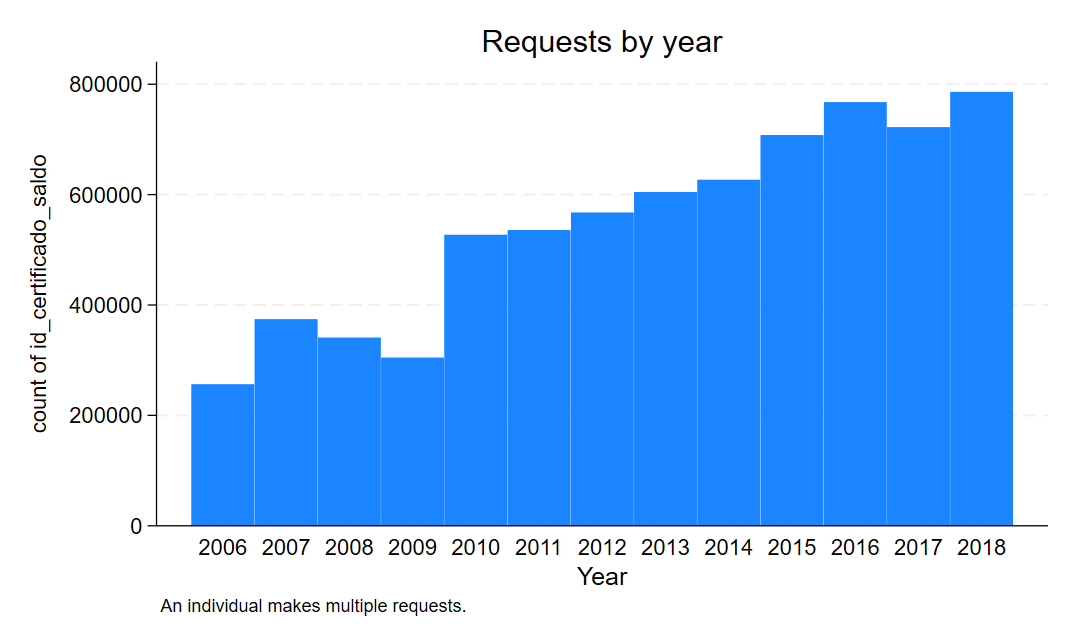
\includegraphics[scale=0.27]{figures/IE0_plot0.png}
\end{tabular}
\end{figure}


Figure \ref{fig:ie0_1} shows the amount of savings of individuals in the sample. Where 1UF is around 40 USD. The distribution is truncated at the 99th percentile of savings. 


\begin{figure}[H]
\caption{}
\label{fig:ie0_1}
\centering{}%
\begin{tabular}{cc}
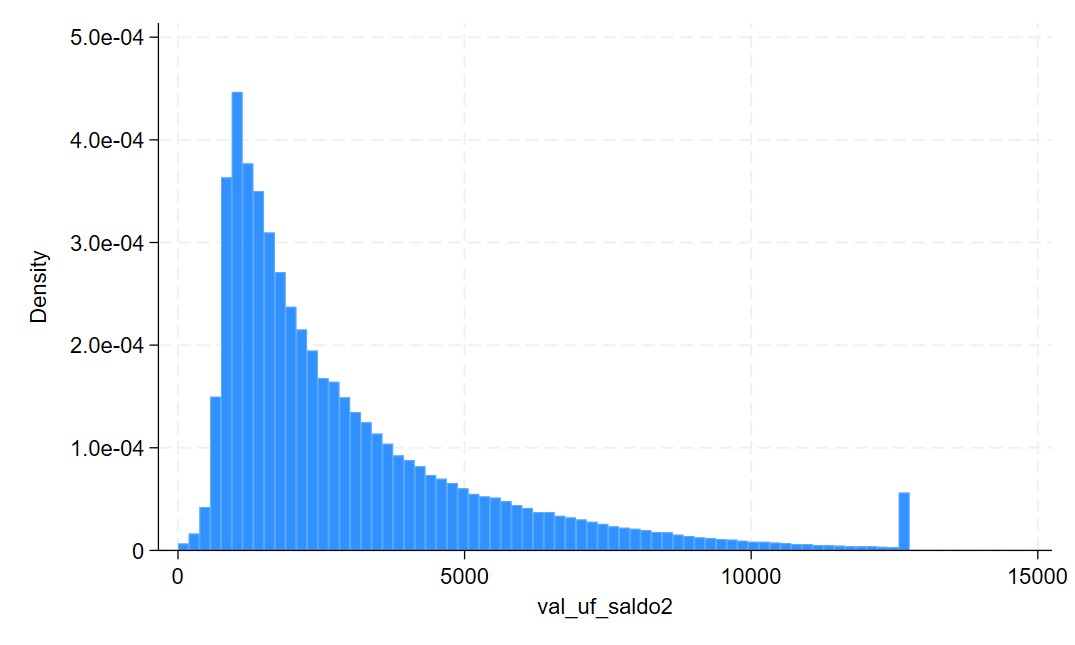
\includegraphics[scale=0.27]{figures/IE0_plot1.png} 
\end{tabular}
\end{figure}



Figure \ref{fig:ie0_2} shows the number of requests for each type of financial product in absolute terms and then their respective shares. The changes are not particularly large, it seems like the share of each financial product is relatively stable over time.

NOTE: ANNUITIES WITH PW(GREEN) START FROM 0 IN 2006 HENCE PROBABLY THEY ARE A FINANCIAL INNOVATION. 

\begin{figure}[H]
\caption{}
 \label{fig:ie0_2and3}
\centering{}%
\begin{tabular}{cc}
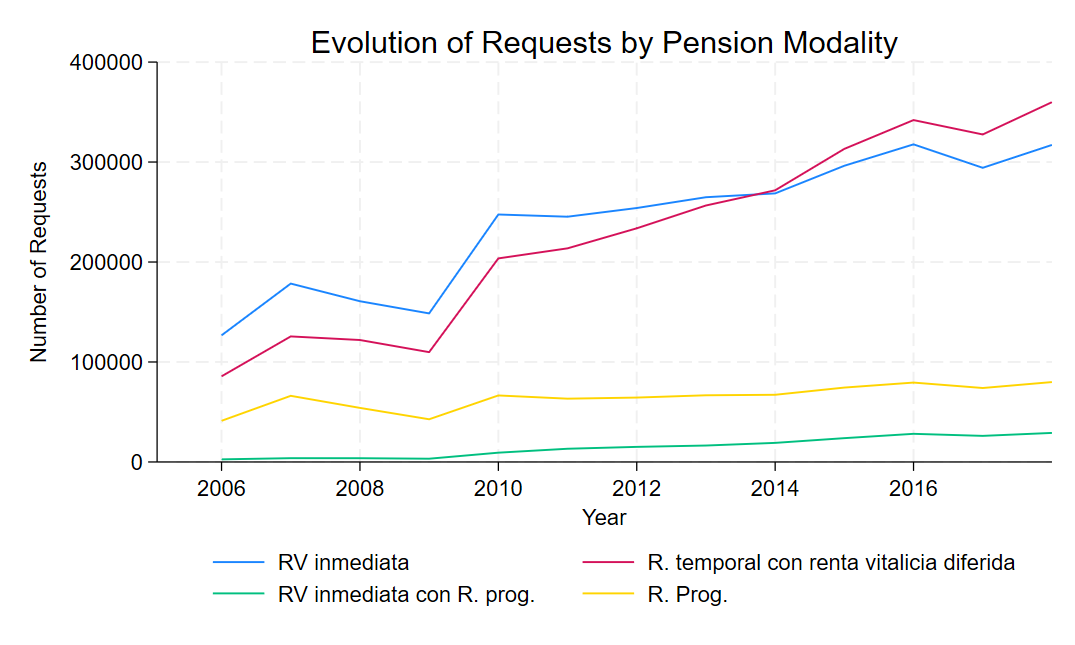
\includegraphics[scale=0.27]{figures/IE0_plot2.png} & 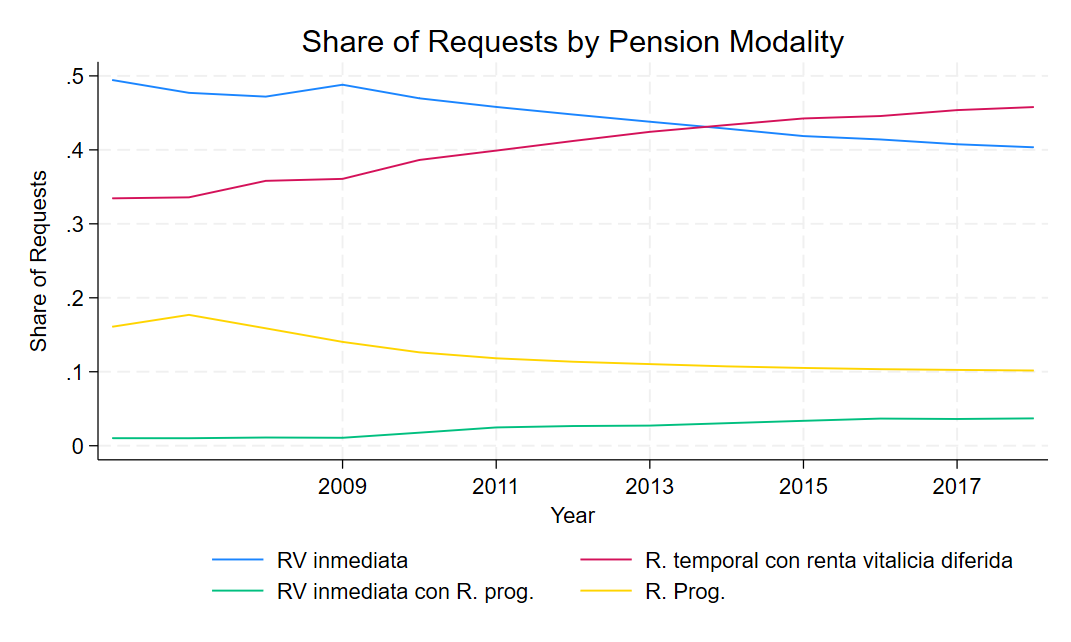
\includegraphics[scale=0.27]{figures/IE0_plot3.png}
\end{tabular}
\end{figure}


Figure \ref{fig:ie0_4} shows the shares for the whole sample as a function of savings. Richer individuals tend to buy more annuities with PW and less PW. This is explained by the fact that there is a minimum amount of savings required to buy an annuity and also could have to do with a higher life expectancy. 


\begin{figure}[H] 
\caption{}
\label{fig:ie0_4}
\centering{}%
\begin{tabular}{cc}
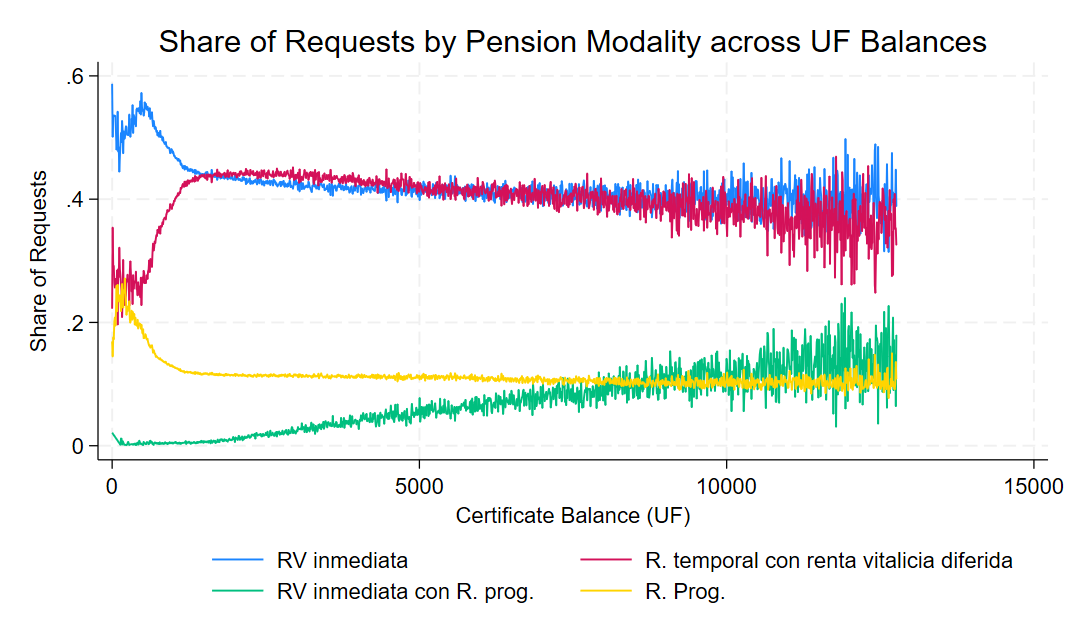
\includegraphics[scale=0.27]{figures/IE0_plot4.png}
\end{tabular}
\end{figure}

Figure \ref{fig:ie0_5} shows how many guaranteed months people buy. 
\begin{figure}[H] 
\caption{}
\label{fig:ie0_5}
\centering{}%
\begin{tabular}{cc}
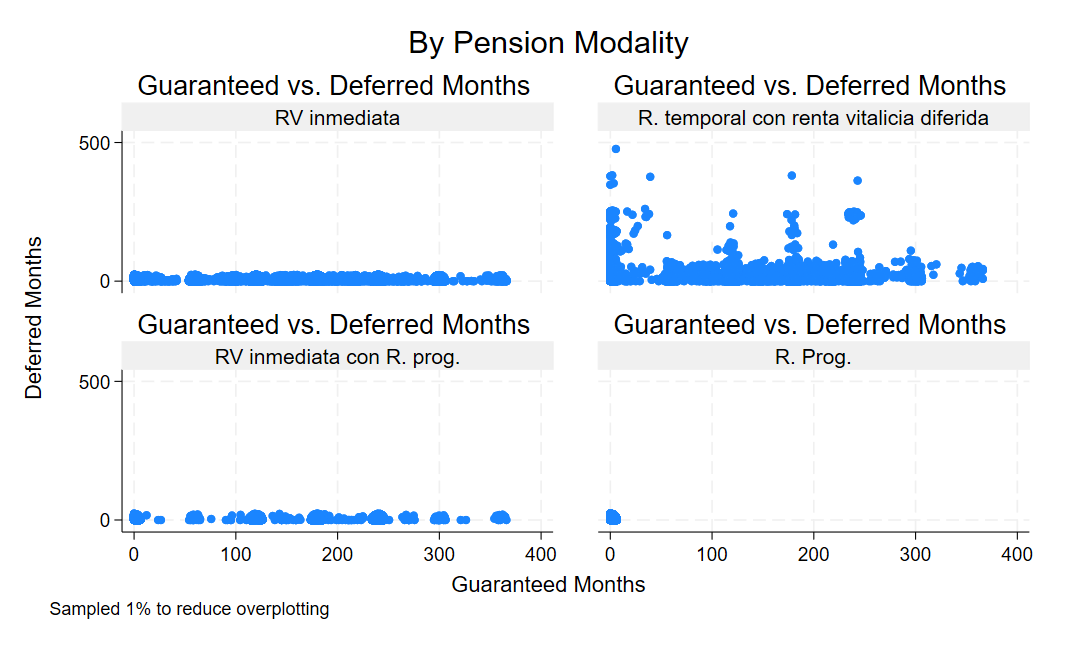
\includegraphics[scale=0.27]{figures/IE0_plot5.png}
\end{tabular}
\end{figure}

\section{IE 1}


Figure \ref{fig:ie1_1} the history of the credit rating for selected insurers.  
\begin{figure}[H]
\caption{}
 \label{fig:ie1_1}
\centering{}%
\begin{tabular}{cc}
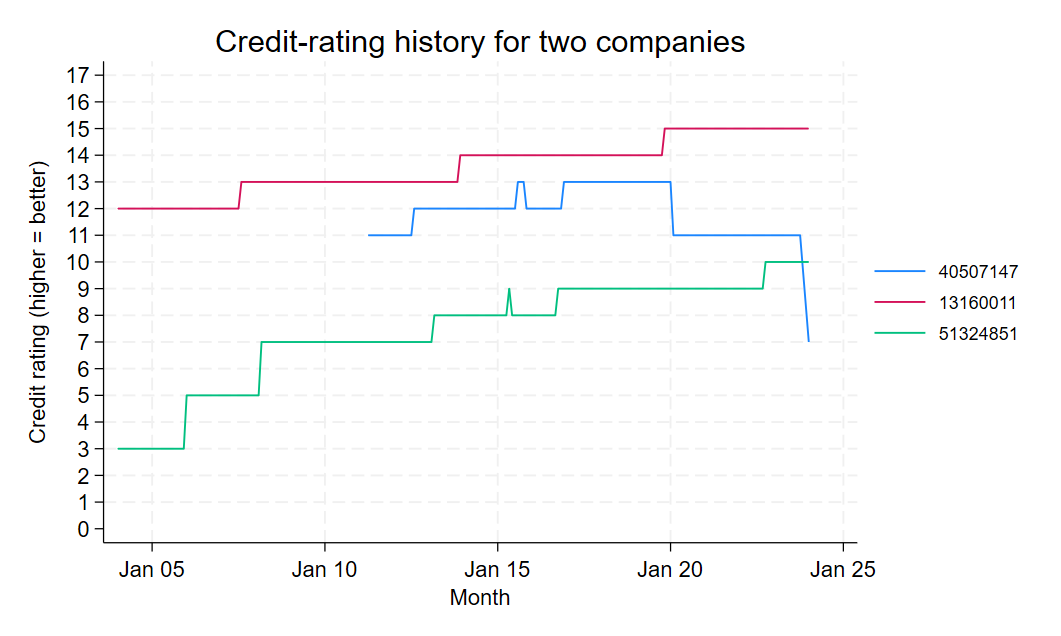
\includegraphics[scale=0.27]{figures/IE1_credit_history.png}
\end{tabular}
\end{figure}

Only 2\% of the offers constitute external offers, because individuals request offers from many financial products (make many requests), then receive many offers (one for each offering company) for each request, and then in case of requesting external offers they do it for only a subset of the initial offers. 

\section{IE 2}

Figure \ref{fig:ie2_1} shows the number of external offers that buyers request.

\begin{figure}[H]
\caption{}
\label{fig:ie2_1}
\centering{}%
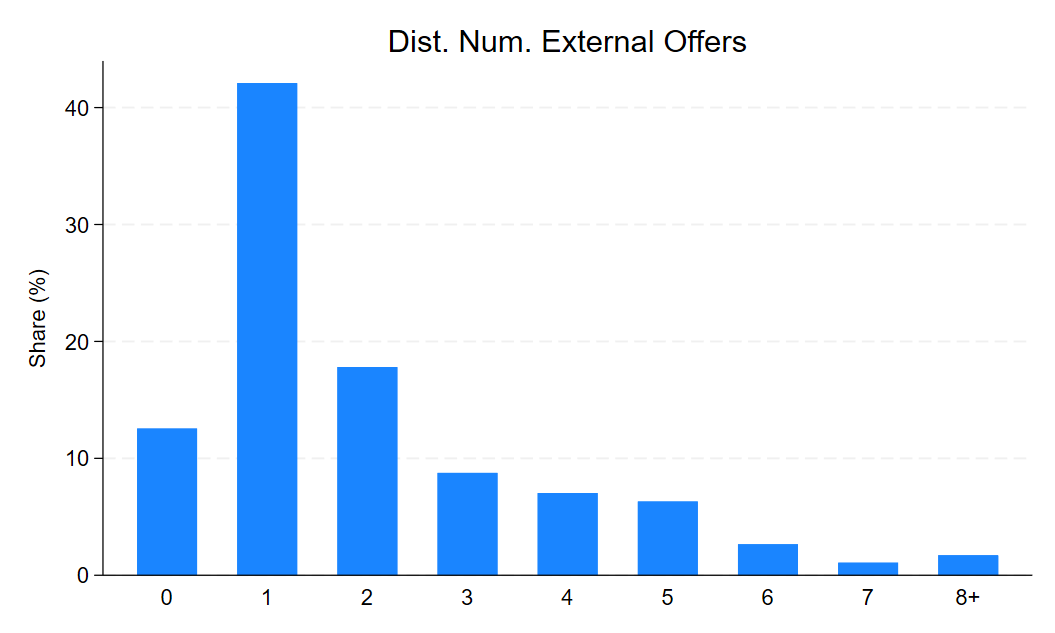
\includegraphics[scale=0.27]{figures/IE2_dist_external_offers.png}
\end{figure}







Figure \ref{fig:ie2_2} shows 


\begin{figure}[H]
\caption{}
 \label{fig:ie2_2}
\centering{}%
\begin{tabular}{cc}
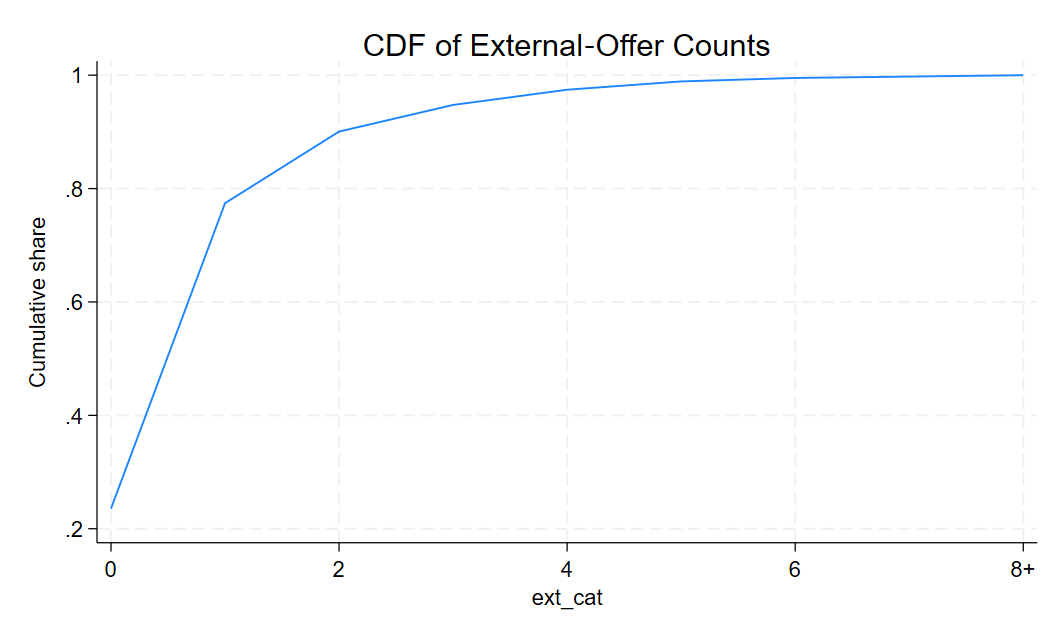
\includegraphics[scale=0.27]{figures/IE2_CDF_number_extoffers.png} &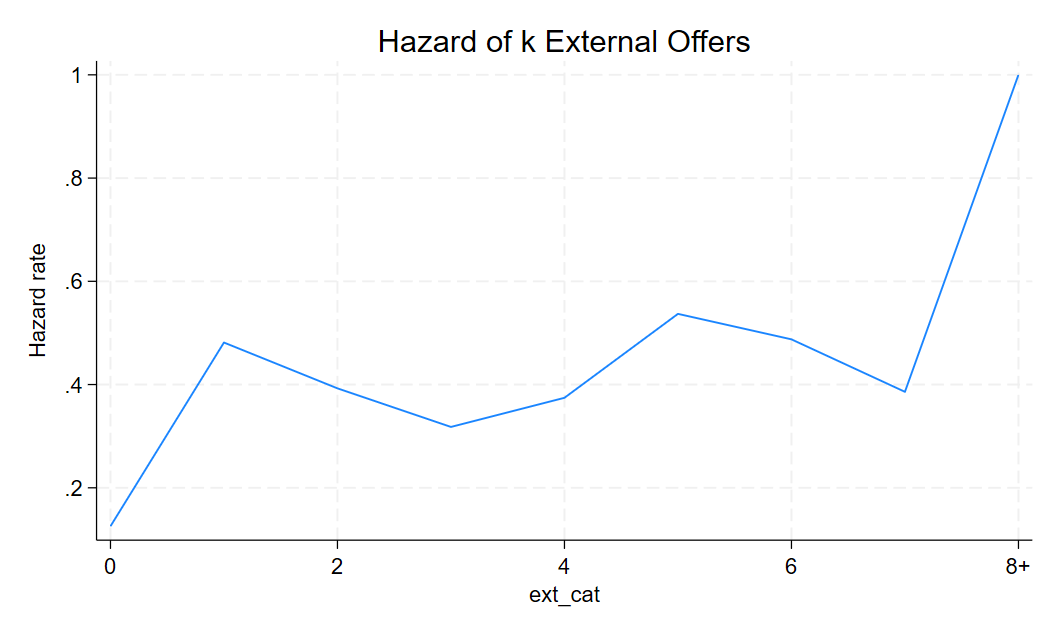
\includegraphics[scale=0.27]{figures/IE2_hazard_number_extoffers.png}
\end{tabular}
\end{figure}



Figure \ref{fig:ie2_3} shows the average number of searches for individuals grouped by their quintile of savings, which is a proxy of income. Specifically an increase of savings by a standard deviation is related to .72 additional searches. 


\begin{figure}[H]
\caption{}
 \label{fig:ie2_3}
\centering{}%
\begin{tabular}{cc}
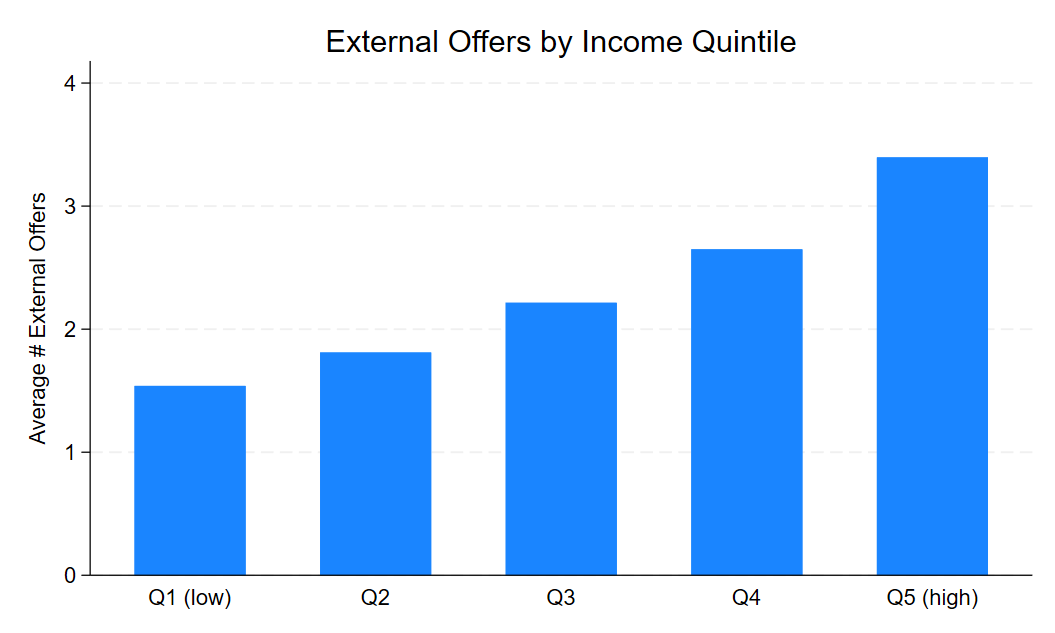
\includegraphics[scale=0.27]{figures/IE2_search_by_income_quintile.png}
\end{tabular}
\end{figure}

Figure \ref{fig:ie2_4} shows the CDF and hazard rate of searches grouped by savings quintile. 

\begin{figure}[H] 
\caption{}
\label{fig:ie2_4}
\centering{}%
\begin{tabular}{cc}
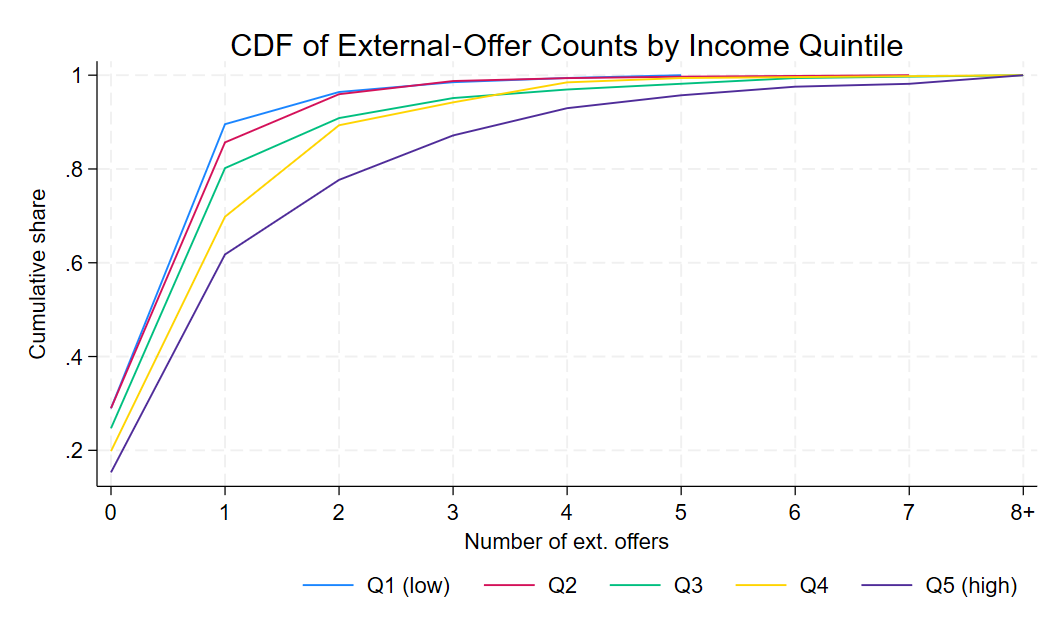
\includegraphics[scale=0.26]{figures/IE2_search_CDF_by_income_quintile.png} & 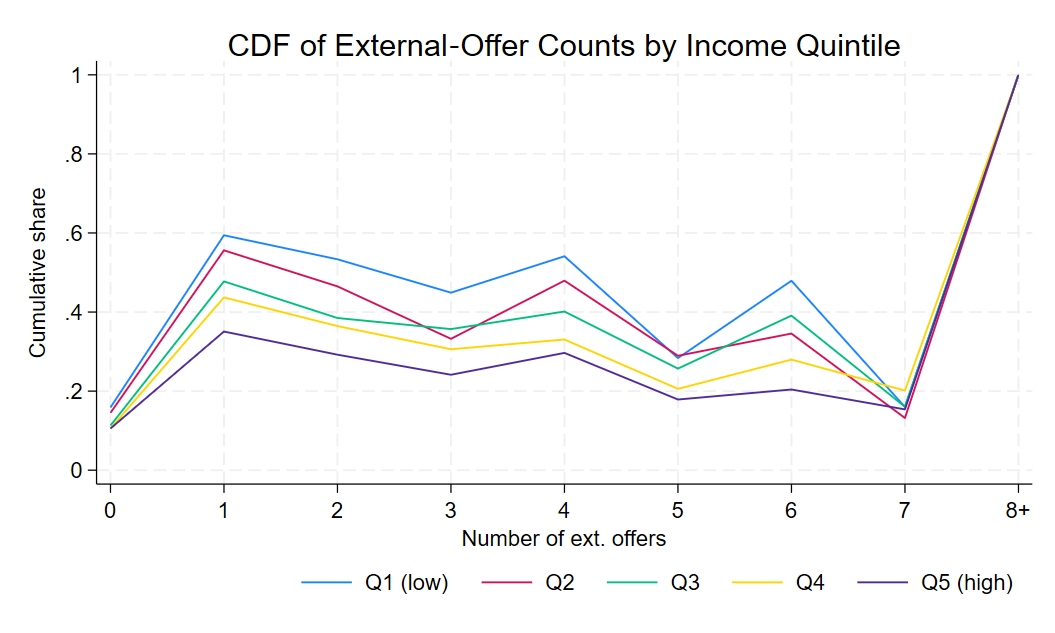
\includegraphics[scale=0.26]{figures/IE2_search_hazardrate_by_income_quintile.png}
\end{tabular}
\end{figure}

\subsection{Dispersion in offers within group}






\end{document}